\documentclass[xcolor=dvipsnames, aspectratio=1610]{beamer}

\usetheme[1610]{ZBH}
\usepackage{graphicx}
\usepackage{algpseudocode}
\usepackage{numprint}
\usepackage[utf8]{inputenc}

\definecolor{greyish}{rgb}{224,224,224}
\setbeamertemplate{blocks}[rounded]
\setbeamercolor{block title}{fg=white,bg=MidnightBlue}
\setbeamercolor{block body}{fg=black,bg=lightgray!50}
       
\author{Meike Bruns, Florian Markowsky, Michael Spohn}
\title{Proteinsequenz-Vergleich mit KSEARCH und SANS}
\date{\today}

\AtBeginSubsection []
 {
  \begin{frame} 
    \frametitle{Gliederung}
    \tableofcontents[currentsection, currentsubsection]
  \end{frame}
}

\begin{document}

\maketitle

\begin{frame}
	\frametitle{Gliederung}
	\tableofcontents
\end{frame}

\section{Einleitung}

\begin{frame}{Sequenzvergleiche}
  \begin{itemize}
    \item Die Bestimmung von Ähnlichkeiten zwischen Sequenzen ist eine häufige Aufgabe bei der Sequenzanalyse 
    \item Exakte Sequenzvergleiche sind oft zu zeitaufwändig 
  \end{itemize}
\end{frame}

\begin{frame}{Sequenzvergleiche - Methoden}
  \begin{itemize}
    \item Alignmentbasierte Methoden
      \begin{itemize}
        \item SSEARCH\\
              \scriptsize ermittelt optimale lokale Alignments mittels Smith-Waterman-Algorithmus                 
        \item \normalsize FASTA\\
              \scriptsize verbindet HotSpots zu approximativen Alignments            
        \item \normalsize BLAST\\
              \scriptsize erweitert Hits zu Maximum Segment Pairs
       \end{itemize}
    \item \normalsize Ranking mittels Feature-Vektoren
      \begin{itemize}
        \item USEARCH\\
              \scriptsize Vorsortieren der Datenbank nach Anzahlen gemeinsamer Substrings, Abbruch der Suche nach erstem    Hit

        \item \normalsize KSEARCH \\
              \scriptsize Bewertet Sequenzpaare aufgrund gemeinsamer k-mere
        \item \normalsize SANS\\
              \scriptsize Bewertet Sequenzpaare aufgrund gemeinsamer Substrings
      \end{itemize}
%      \item Aufgrund interesting similarities extend higher levels of mismathches sind Proteinanalysen mit suffixarrays nicht so verbreitet
  \end{itemize}
\end{frame}

\begin{frame}{SANS \& KSEARCH}
  \begin{itemize}
    \item Entwickelt von J. Patrik Koskinen \& Liisa Holm
    \item Paper: "SANS: high-throughput retrieval of protein sequences allowing 50\% mismatches" 
    \item Suffixarray-basierte Methoden zur Sequenzähnlichkeitsanalyse von Proteinen
    \item Koskinen \& Holm finden für ihre Tools eine mit Blast vergleichbare Sensitivität für Proteinpaare mit 50-100\% Sequenzidentität
    \item Tools zum Download unter 
  \end{itemize}
\end{frame}

\section{Algorithmen \& Implementierung}

\subsection{Datenstrukturen}

\begin{frame}{Suffixarrays}
  \begin{itemize}
    \item Enthalten alle Suffixe einer Sequenz in lexikographischer Ordnung
  \end{itemize}
  \begin{block}{Beispiel}
    \begin{columns}
      \column{.4\textwidth}
        Sequenz = GYBLAAB\$
      \scriptsize\column{.5\textwidth}
        Suffixarray:\\
        AAB\$\\
        AB\$\\
        BLAAB\$\\
        B\$\\
        GYBLAAB\$\\
        LAAB\$\\
        YBLAAB\$\\
        \$\\
      \normalsize
    \end{columns}
  \end{block}
\end{frame}

\begin{frame}{Rot-Schwarz-Bäume}
  \begin{itemize}
    \item Binäre Bäume
    \item Durch rot-schwarz-Eigenschaften balanciert:
      \begin{itemize}
        \item Knoten sind rot oder schwarz, die Wurzel ist immer schwarz
        \item Jeder Pfad von einem Knoten x zu einem Blatt enthält die gleiche Anzahl schwarzer 
        Knoten
        \item Es folgen keine 2 roten Knoten aufeinander  
      \end{itemize}
    \item Ermöglichen schnelles Einfügen und Suchen auf sortierten Daten
  \end{itemize}
\end{frame}

\subsection{KSEARCH}

\begin{frame}{KSEARCH - Berechnen der Scores}
  \begin{equation*}
    KSEARCH(query,database) = \sum_{w \in \mathcal A^k} G_k(query)(w) \cdot G_k(database)(w)
  \end{equation*}  
  \begin{block}{Beispiel}
    \begin{columns}
    \column{.4\textwidth}
    query = BITQAPS\\
    database = PQAPSQAP\\  
    \column{.5\textwidth}  
    \scriptsize\begin{tabular}{cccc}
    kmer & query & database & Produkt\\
    APS & 1 & 1 & 1\\
    BIT & 1 & 0 & 0\\
    ITQ & 1 & 0 & 0 \\
    PQA & 0 & 1 & 0\\
    PSQ & 0 & 1 & 0\\
    QAP & 1 & 2 & 2\\
    SQA & 0 & 1 & 0\\
    TQA & 1 & 0 & 0\\    
    \end{tabular}
    \normalsize
    \end{columns}
  \end{block}
\end{frame}

\begin{frame}{Notation}
  \begin{itemize}
    \item $Q$ bzw. $D$ - Menge der Query- bzw. Datenbank-Proteine
    \item $q$ bzw. $d$ - ein Query- bzw. Datenbank-Protein
    \item $|Q|$ bzw. $|D|$- Anzahl der Query- bzw. Datenbank-Proteine
    \item $|q|$ bzw. $|d|$ - Länge eines Query- bzw. Datenbank-Proteins
    \item $|q_0..q_n|$ bzw. $|d_0..d_n|$ - Länge aller konkatenierten Query- bzw. Datenbank-Proteine
    \item $kVariety(q)$ bzw. $kVariety(d)$ - Anzahl untersciedlicher kmere in einem Query- bzw. Datenbank-Protein
  \end{itemize}
\end{frame}

\begin{frame}{KSEARCH}
 \begin{algorithmic}
   \Function{KSEARCH}{query-proteins $Q$, database-proteins $D$}
      \For{each query-protein $q$}  
        \State calculate kmer-profile \Comment $O(|q|)$
        \State store kmer-profile in hashtable
      \EndFor \Comment $\boldsymbol{O(|q_0..q_n|)}$
       \For{each database-protein $d$} 
         \State calculate kmer-profile \Comment $O(|d|)$
         \For{i in $Q$}
           \State calculate $KSEARCH(d,q_{i})$ \Comment $O(kVariety(d))$   
           \State output $KSEARCH(d,q)$
         \EndFor \Comment $\boldsymbol{ O(|Q| \cdot kVariety(d))}$
       \EndFor   \Comment $\boldsymbol{O(|d_0..d_n|+|D| \cdot |Q| \cdot kVariety(d))}$  
    \EndFunction \Comment overall time complexity: $\boldsymbol{O(|q_0..q_n|+|d_0..d_n|+|D| \cdot |Q| \cdot kVariety(d))}$

  \end{algorithmic}
\end{frame}

\begin{frame}{Implementierungsansatz und Analyse}
  \begin{itemize}
    \item Koskinen \& Holm
      \begin{itemize}
        \item Berechnung des KSEARCH-Scores mittels Suffixarrays
      \end{itemize}
    \item MMF
      \begin{itemize}
        \item Berechnung der KSEARCH-Scores mittels gehashter k-mer-Profile
      \end{itemize}
    \end{itemize}
    
  \begin{tabular}{|l|c|c|}
     \hline
     & Koskinen \& Holm & MMF\\ 
     \hline
    Laufzeitkomplexität & $O(|d_0..d_n| \cdot |q_0..q_n|)$ & $O(|q_0..q_n|+|d_0..d_n|+|D| \cdot |Q| \cdot kVariety(d))$\\
    \hline
    Speicherplatzbedarf & keine Angabe & $O(|Q| \cdot |D|+ |Q| \cdot kVariety(q))$ \\
    \hline
  \end{tabular}
\end{frame}

\begin{frame}{Optimierungsmöglichkeiten/Probleme KSEARCH}
  \begin{itemize}
    \item k-mer Profile zunächst als Matrix gespeichert: zu hoher Speicherbedarf
    \item Implementierung mit doppelter For-Schleife: zu hohe Laufzeit
    \item Lösung: hashing von vorhandenen kmeren
  \end{itemize}
\end{frame}

\subsection{SANS}

\begin{frame}{SANS - Berechnen der Scores}
  \begin{itemize}
    \item Substrings von Sequenzen, die im Suffixarray nebeneinander liegen, haben typischerweise lange gemeinsame Präfixe
    \item  SANS-Scores bewerten Proteinpaare aufgrund von Nachbarschaften im Suffixarray
  \end{itemize}
\end{frame}

\begin{frame}{SANS - Berechnen der Scores}
  \begin{block}{SANS}
  \begin{figure}
        \includegraphics<1>[width=0.4\textwidth]{SANS1.jpg}
        \includegraphics<2>[width=0.4\textwidth]{SANS2.jpg}
        \includegraphics<3>[width=0.4\textwidth]{SANS3.jpg}
    \end{figure} 
  \end{block}
\end{frame}

\begin{frame}{SANS}
 \begin{algorithmic}
   \Function{SANS}{$query proteins Q, database proteins D, windowsize h$}
     \State calculate $suffixarray_Q$ for query proteins \Comment $O(|d_0..d_n|)$
     \State calculate $suffixarray_D$ for database proteins \Comment $O(|q_0..q_n|)$
     \State initialize score matrix \Comment $O(|Q|\cdot|D|)$
     \State initialize $position = 0$
     \For{each $suffix_{qx}$ from 0 - $suffixarray_Q$.length}
       \State  $position$ = \Call {findPosition}{$suffix$, $suffixarray_D$, $position$} 
       \State shift $2h$ window over $position$ 
       \For{each $suffix_{dx}$ in window}
         \State update SANS-scores for  $(q_x,d_x)$
       \EndFor \Comment $\boldsymbol{O(2h)}$
     \EndFor \Comment $\boldsymbol{O(|q_0..q_n|\cdot2h + |d_0..d_n|)}$
    \EndFunction  \Comment overall time complexity: $\boldsymbol{O(|q_0..q_n|\cdot2h + |d_0..d_n|+|Q|\cdot|D|)}$ 
  \end{algorithmic}
\end{frame}

\begin{frame}{findPosition}
  \begin{algorithmic}
    \Function{findPosition}{$suffix$, $suffixarray_D$, $position$}
      \For{$i$ in $position$..$suffixarray_D$.length}
        \If{$suffix$ fits in $suffixarrax_D[i]$}
          \State return $i$ 
        \EndIf
      \EndFor 
    \EndFunction
  \end{algorithmic} 
\end{frame}

\begin{frame}{Implementierungsansatz und Analyse}
  \begin{itemize}
    \item Koskinen \& Holm
      \begin{itemize}
        \item Ermitteln der Positionen durch Mergen der Suffixarrays
      \end{itemize}
    \item Unsere Implementierung
      \begin{itemize}
        \item Ermitteln der Positionen durch for-Schleifen
      \end{itemize}
  \end{itemize}
    \begin{tabular}{|l|c|c|}
     \hline
     & Koskinen \& Holm & MMF\\ 
     \hline
    Laufzeitkomplexität & $O(|d_0..d_n| + |q_0..q_n|)$ & $O(|q_0..q_n|\cdot2h + |d_0..d_n|+|Q|\cdot|D|)$\\
    \hline
    Speicherplatzbedarf & keine Angabe & $O(|Q| \cdot |D|+|d_0..d_n| + |q_0..q_n|))$ \\
    \hline
  \end{tabular}
\end{frame}

\begin{frame}{Optimierungsmöglichkeiten SANS}
  \begin{itemize}
    \item Mergen der Suffixarrays statt for-schleifen:\\
          Speicherplatzersparnis: Statt der gesamten Suffixarrays nur den window-Bereich im Arbeitsspeicher vorhalten    
  \end{itemize}
\end{frame}

\subsection{Software Architektur}

\begin{frame}{Genometools}
  \begin{itemize}

    \item Wir implementieren in der Softwareumgebung Genometools, aus der wir eine Anzahl an Tools und Klassen nutzen:
    \begin{itemize}
      \item encseq encode - Tool zum codieren von Sequenzen 
      \item suffixerator - Tool zur Berechnung von Suffixarrays aus Sequenz-Dateien oder encseqs
      \item encseq - effizienter Datentyp für Sequenzen
      \item kmer iterator - Klasse zur Iteration über kmere von encseqs
      \item hashmap - Klasse zum Anlegen von Hashes
      \item ranked list - Rot-Schwarz-Baum basierte Liste

    \end{itemize}    
  \end{itemize}
\end{frame}


\begin{frame}{Ausgabemöglichkeiten von KSEARCH \& SANS}
  \begin{itemize}
    \item -matrix 
      \begin{itemize}
        \item Gibt alle Scores aus
      \end{itemize}           
    \item -threshold x 
      \begin{itemize}
        \item  Gibt alle Scores über einem Threshold x aus
      \end{itemize}
    \item -nbest x
      \begin{itemize}
        \item  Gibt die x besten Scores aus
      \end{itemize} 
  \end{itemize}
\end{frame}

\begin{frame}{Seqscore Toolbox}
  \begin{figure}[h]
    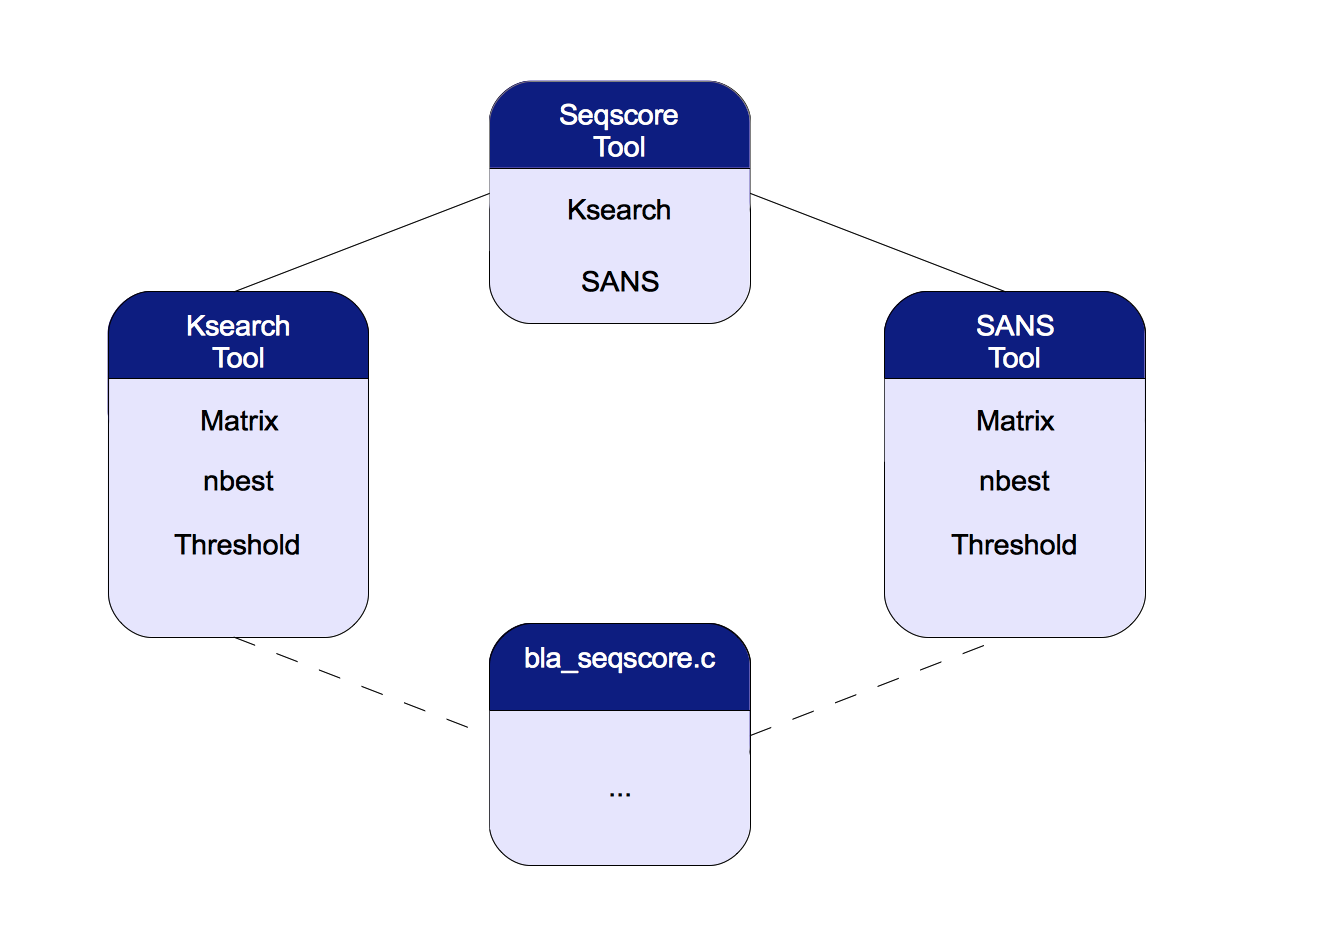
\includegraphics[height=7cm]{img/dia1.png}
  \end{figure}
\end{frame}

\begin{frame}{bla\_seqscore.c}
  \begin{figure}[h]
    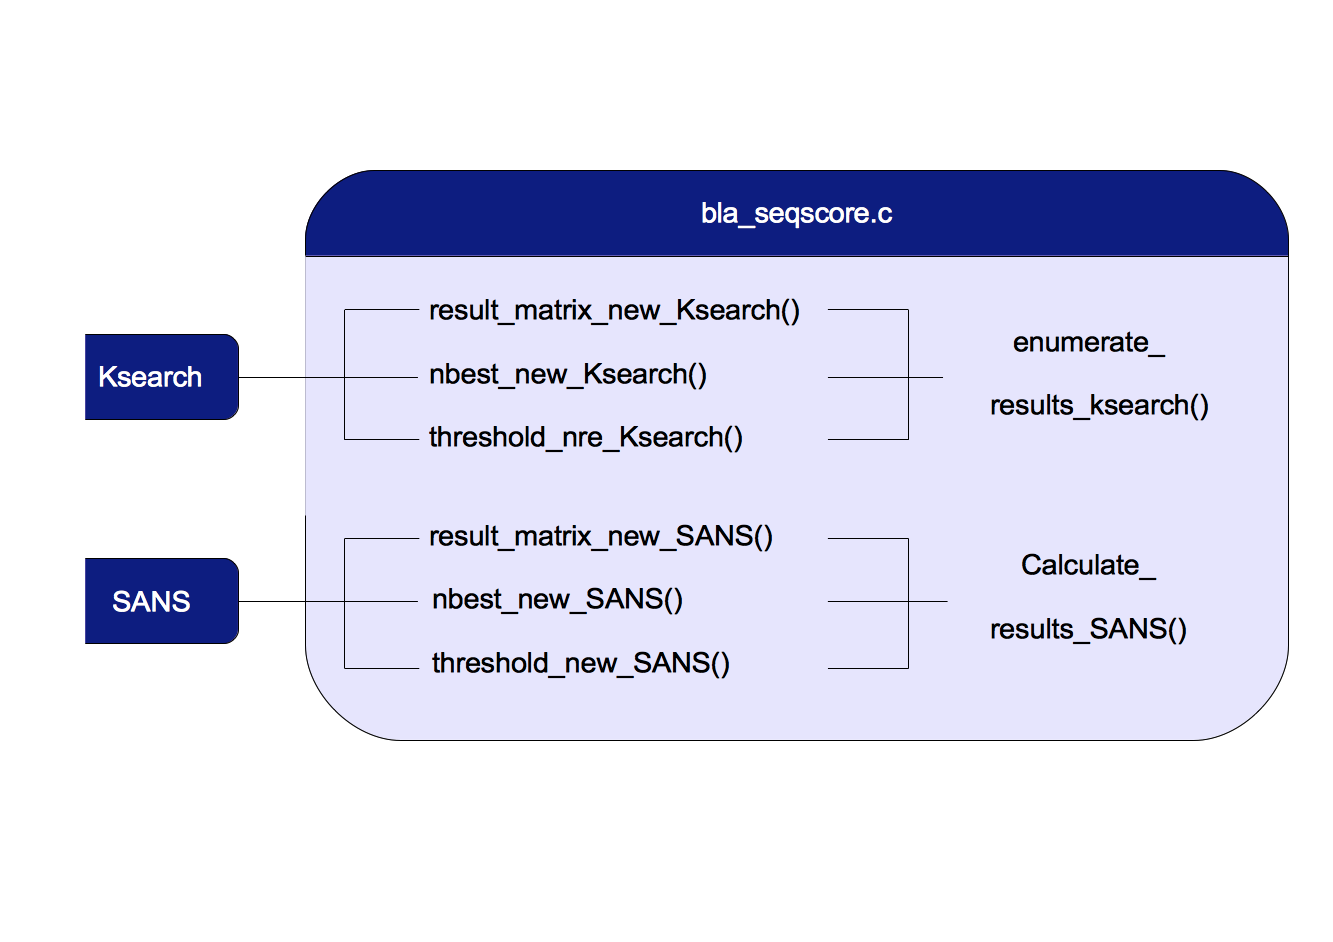
\includegraphics[height=7cm]{img/dia2.png}
  \end{figure}
\end{frame}

\begin{frame}{Berechnungs-Aufruf}
  \begin{figure}[h]
    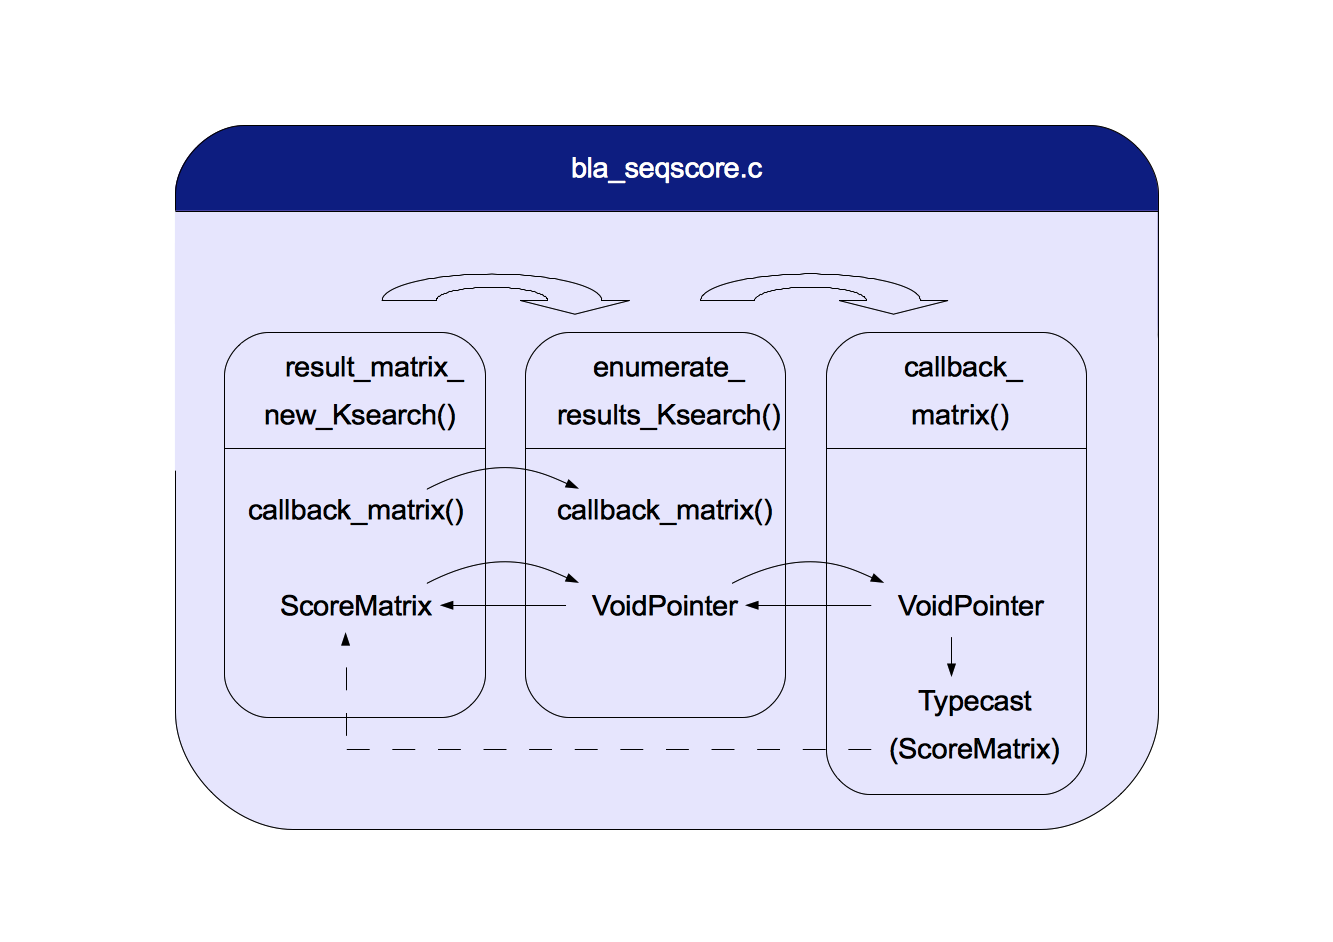
\includegraphics[height=7cm]{img/dia3.png}
  \end{figure}
\end{frame}

\section{Auswertung}
  \begin{frame} 
    \frametitle{Gliederung}
    \tableofcontents[currentsection]
  \end{frame}

\begin{frame}{Laufzeiten}
  \begin{itemize}
    \item Query: 1083 Rattus rattus Proteine von NCBI \tiny{\url{http://www.ncbi.nlm.nih.gov/protein}}
    \item \normalsize{Database: Swissprot-Datenbank} \tiny{\url{http://www.uniprot.org/downloads}}
  \end{itemize}
  \begin{tabular}{l|cc}
    Algorithmus & Indexing & Suche \\
    \hline
    KSEARCH Holms k6 & 1m29s & 0m14s \\
    KSEARCH MMF k6 & -  & 511m53s \\
     SANS Holms h16 & 1m29s &  0m15s \\
       SANS MMF  h16 & 14m19s & 0m36s \\
  \end{tabular}
\end{frame}

\begin{frame}{Sensitivitaet}
  Hier kommt eine Sensitivity-Grafik wie die im Paper hin.
\end{frame}

\begin{frame}{AUC}
  Hier kommt eine AUC-Grafik hin
\end{frame}

\end{document}
